\documentclass{llncs}
\usepackage{makeidx}
\usepackage{graphicx}
\DeclareGraphicsExtensions{.pdf,.png,.jpg}
\usepackage{wrapfig}
\usepackage{subfig}
\usepackage{caption}
\usepackage{colortbl}
\usepackage{booktabs}
\usepackage{datatool}
\usepackage[table]{xcolor}
\usepackage{siunitx}
\usepackage{pgfplots}
\usepackage{float}
\usepackage{url}
\pgfplotsset{footnotesize,compat=1.8}
\usepackage{listings}
\lstset{frame=tbrl, aboveskip=1mm, belowskip=1mm, showstringspaces=false, columns=flexible, basicstyle={\scriptsize\ttfamily}, breaklines=true, tabsize=3}

%Striped tables 
\definecolor{light-gray}{gray}{0.9}
\let\stripedtabular\tabular
\let\endstripedtabular\endtabular
\renewenvironment{stripedtabular}{\rowcolors{0}{black!20}{black!5}\tabular}{\endtabular}

\hyphenation{equal-ly}

%Load data
\DTLloaddb{examplesdata}{examplesdata.csv}
\DTLloaddb{mutateddata}{mutateddata.csv}
\DTLloaddb{generateddata}{generateddata.csv}

%Anti-American-hegemony package
\usepackage[utf8]{inputenc}

\title{General Video Game Evaluation Using Relative Algorithm Performance Profiles}
\author{
Thorbjørn S. Nielsen, Gabriella A. B. Barros, Julian Togelius, Mark J. Nelson\\
}
\institute{
Center for Computer Games Research, IT University of Copenhagen, Denmark
}

\begin{document}

\maketitle

\begin{abstract}
In order to generate complete games through evolution we need generic and reliably evaluation functions for games. It has been suggested that game quality could be characterised through playing a game with different controllers and comparing their performance. This paper explores that idea through investigating the relative performance of different general game-playing algorithms. Seven game-playing algorithms was used to play several hand-designed, mutated and randomly generated VGDL game descriptions. Results discussed appear to support the conjecture that well-designed games have, in average, a higher performance difference between better and worse game-playing algorithms.
%\keywords{VGDL, }
\end{abstract}

%Responsibilities
%Thorbjørn: get data, produce tables, answer questions
%Gabriella: coordinate paper writing, describe methods and results, make sure things happen
%Julian: write intro, background, conclusion, discussion
%Mark: help Julian write background/discussion, language edit the whole paper

\section{Introduction}
How well do knowledge-free algorithms play really bad video games? This might not be a question that has kept you awake at night, but as we shall show there are excellent reasons to consider it. Reasons having to do with understanding fundamental design characteristics of a broad class of simple video games, and laying the groundwork for automatically generating such games.

One way to generate complete games is to search a space of games represented in a programming language like C or Java, however the subset of games with well-formed rules can be increased by using a game description language (GDL). The search could be done with e.g. evolutionary computation, starting with a population of randomly generated games and/or hand-designed games, and applying generation after generation of mutation and recombination, keeping the better game and replacing the worse games. Eventually such a process is likely to come up with good games that no-one has ever seen before.

But this supposes that we have a way of automatically telling good games from bad games (or not-quite-so-bad games from really bad games). In other words, we need a fitness function. Part of the fitness function could consist in inspecting the rules as expressed in the GDL, e.g. to make sure that there are winning conditions which could in principle be fulfilled. But there are many bad games that fulfil such criteria. To really understand a game, you need to play it. It seems the fitness function therefore needs to incorporate a capacity to play the games it is evaluating.

This game-playing capacity needs to be \emph{general}, because we know almost nothing about the games that will be evaluated. We can therefore not incorporate any domain knowledge about these games; we need algorithms that are as \emph{knowledge-free} as possible. Examples of such algorithms are the various tree-search algorithms, such as Minimax and Monte Carlo tree search (MCTS), that have been widely used for playing various games. But online evolutionary algorithms might also be used as knowledge-free algorithms. In case a heuristic representing the quality of a particular in-game state is need, such a heuristic should be as neutral as possible, e.g. the score of the game.

Just being able to play a game does not in itself tell us how good the game is. Many boring games are perfectly playable by an algorithm. And because we don't know the game, we don't know what constitutes good or bad play, compared to how well or badly the game could be played. However, the relative performance of different game-playing algorithms might tell us something about a game. Good games are likely to have high skill differentiation: good players get better outcomes than bad players. We therefore formulate the following hypothesis: the performance difference (measured as score and/or win-rate) between generally better game-playing algorithms and generally worse game-playing algorithms is on average higher for well-designed games than for poorly designed games. But there might very well be other interesting differences between classes of games that can be discerned by looking at the performance profiles of sets of game-playing algorithms.

We carry out this investigation using the General Video Game Playing platform (GVG-AI) and its associated Video Game Description Language (VGDL). This framework makes 20 hand-designed games available, mostly versions of well-known arcade games. We contrast those games with a large number of randomly generated games in the same language, and with a large number of ``mutations'' of the hand-designed games. A core assumption we make is that the hand-designed games are, on average, better designed than the randomly generated ones. We calculate a performance profile using several game-playing algorithms available in the GVG-AI framework and some new algorithms. The concrete contributions of this paper thus include two new variations on Monte Carlo-based game-playing, as well as a quantitative investigation of the performance profiles of these algorithms and the associated methodology for performing this study. However, we primarily see this work as groundwork for a reliable game fitness function, that will eventually allow us to generate good new sets of game rules.

%---------------------------------------------------------------

\section{Background}
%Julian and Mark
The idea of generating complete games through algorithms is not itself new. The problem in full generality is quite large, so usually a subset of the general problem is tackled. Videogames may be comprised of a large number of tangible and intangible components, including rules, graphical assets, genre conventions, cultural context, controllers, character design, story and dialog, screen-based information displays, and so on~\cite{cook2014angelina,liapis2014creativity,nelson2007automated}.

In this paper we look specifically at generating game rules; and more specifically the rules of arcade-style games based on graphical movement and local interaction between game elements, represented in VGDL. The two main approaches that have been explored in generating game rules are reasoning through constraint solving~\cite{smith2010variations} or search through evolutionary computation or similar forms of stochastic optimisation~\cite{togelius2008experiment,browne2008automated,font2013towards}. In either case, rule generation can be seen as a particular kind of procedural content generation~\cite{pcgbook:ch6}.

It is clear that generating a set of rules that makes for an interesting and fun game is a hard task. The arguably most successful attempt so far, Browne's Ludi system, managed to produce a new board game of sufficient quality to be sold as a boxed product~\cite{browne2008automated}. However, it succeeded partly due to restricting its generation domain to only the rules of a rather tightly constrained space of board games. A key stumbling block for search-based approaches to game generation is the fitness/evaluation function. This function takes a complete game as input and outputs an estimate of its quality. Ludi uses a mixture of several measures based on automatic playthrough of games, including balance, drawishness and outcome uncertainy. These measures are well-chosen for two-player board games, but might not transfer that well to video games or single-player games, which have in a separate analysis been deemed to be good targets for game generation~\cite{togelius2014characteristics}. Other researchers have attempted evaluation functions based on the learnability of the game by an algorithm~\cite{togelius2008experiment} or an earlier and more primitive version of the characteristic that is explored in this paper, performance profile of a set of algorithms~\cite{font2013towards}.

\subsection{Game description languages}

Regardless of which approach to game generation is chosen, one needs a way to represent the games that are being created.\footnote{See \cite{pcgbook:ch6} for a discussion of game-rule representation choices.} For a sufficiently general description of games, it stands to reason that the games are represented in a reasonably generic language, where every syntactically valid game description can be loaded into a specialised game engine and executed. There have been several attempts to design such GDLs. One of the more well-known is the Stanford GDL, which is used for the General Game Playing Competition~\cite{genesereth2005general}. That language is tailored to describing board games and similar discrete, turn-based games; it is also arguably too verbose and low-level to support search-based game generation. The various game generation attempts discussed above feature their own GDLs of different levels of sophistication; however, there has not until recently been a GDL for suitably large space of video games.

\subsection{VGDL}
The Video Game Description Language (VGDL) is a GDL designed to express 2D arcade-style video games of the type common on hardware such as the Atari 2600 and Commodore 64. It can express a large variety of games in which the player controls a moving avatar (player character) and where the rules primarily define what happens when objects interact with each other in a two-dimensional space. VGDL was designed by a set of researchers~\cite{levine2013general,ebner2013towards} (and implemented by Schaul ~\cite{schaul2013video}) in order to support both general video game playing and video game generation.
The language has an internal set of classes, properties and types that each object can defined by.

Objects have physical properties (i.e. position, direction) which can be altered either by the properties defined, or by interactions defined between specific objects. A VGDL description has four parts: the SpriteSet, which defines the ontology of the game -- which sprites exist and what can they do; the LevelMapping, which maps from level description to game state; the InteractionSet, which defines what happens when sprites overlap, and the TerminationSet which defines how the game can be won or last.


\subsection{The GVG-AI Framework}

The GVG-AI framework is a testbed for testing general game-playing controllers against games specified using VGDL. Controllers are called once at the beginning of each game for setup, and then once per clock tick to select an action. Controllers do not have access to the VGDL descriptions of the games. They receive only the game's current state, passed as a parameter when the controller is asked for a move. However these states can be forward-simulated to future states. Thus the game rules are not directly available, but a simulatable model of the game can be used.

The framework additionally contains 20 hand-designed games, which mostly consist of interpretations of classic video games. Each game is also accompanied by five different levels. Figure \ref{fig:vgdl} shows the VGDL description of the game \emph{Missile Command}.


\begin{figure}[!ht]
\centering
\begin{lstlisting}
BasicGame
	SpriteSet
		city  > Immovable color=GREEN img=city
		explosion > Flicker limit=5 img=explosion
		movable >
			avatar  > ShootAvatar stype=explosion
			incoming >
				incoming_slow  > Chaser stype=city color=ORANGE speed=0.1
				incoming_fast  > Chaser stype=city color=YELLOW speed=0.3

	LevelMapping
		c > city
		m > incoming_slow
		f > incoming_fast
		
	InteractionSet
		movable wall  > stepBack
		incoming city > killSprite
		city incoming > killSprite scoreChange=-1
		incoming explosion > killSprite scoreChange=2

	TerminationSet
		SpriteCounter stype=city   win=False
		SpriteCounter stype=incoming win=True
\end{lstlisting}
\caption{Example of VGDL description - a simple implementation of the game Missile Command}
\label{fig:vgdl}
\end{figure}

%image of vgdl description(s)
%image of vgdl games

%---------------------------------------------------------------

\section{Method}
%Gabriella
This section describes the processes used to generate VGDL descriptions, and the expiremental setup in testing the resulting games. First, it will describe the set of human-defined games and controllers used during generation and testing. Then, the two different generation method will be discussed: One that generated descriptions randomly, within certain constraints, and one that tries to mutate existing games into new ones.

\subsection{Example games}
\label{method:examples}
Two of the 20 games from the GVG-AI framework were deemed too monotonous after initial tests. 
In these two games the controllers all had similar scores for each run - or with only one controller being able to increase its score.
The remaining 18 hand-designed VGDL game descriptions were chosen to be used as a baseline for testing and game generation. 
Most of the games are inspired by classic arcade- and Atari games (e.g. Boulderdash, Frogger, Missile Command and Pacman), while some are original creations by the General Video-Game AI Competition's organizers. 

The games can in general be described as action arcade games, in that the player controls a single avatar which must be moved quickly around in a 2D-setting to win, or to get a high score (the player is able to increment a score  counter in all of the games).

\begin{figure}[!ht]
	\subfloat{%\emph{Zelda}\label{subfig-2:dummy}]{%
      		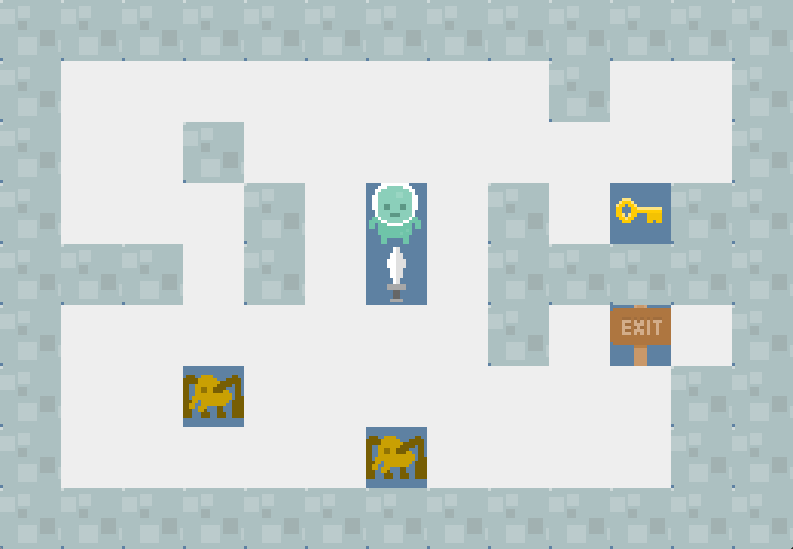
\includegraphics[scale=0.18]{zelda.png}
    	}
	\hfill
	\subfloat{%[\emph{Portals}\label{subfig-1:dummy}]{%
		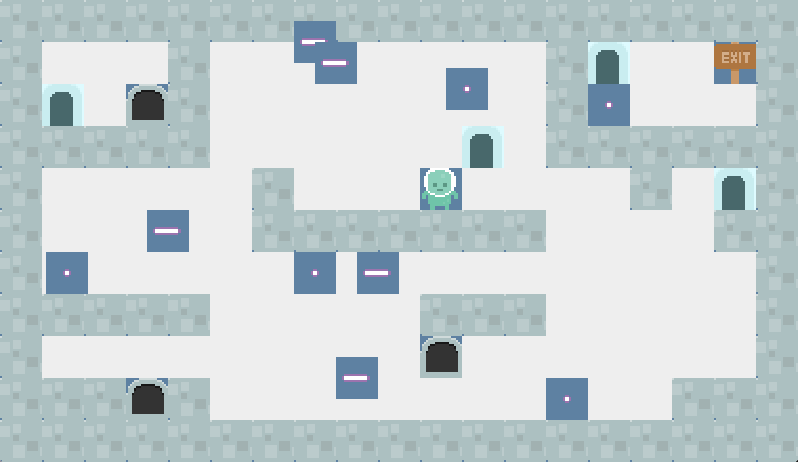
\includegraphics[scale=0.24]{portals.png}
	}\\
	\subfloat{%\emph{Boudlerdash}\label{subfig-2:dummy}]{%
      		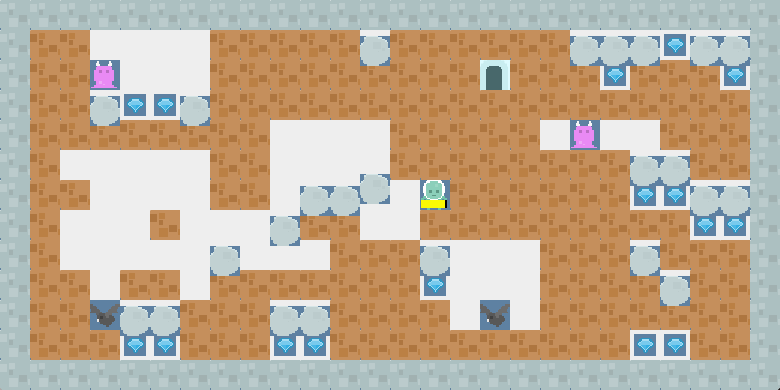
\includegraphics[width=\textwidth]{boulderdash.png}
    	}
    	\caption{A visual representation of a few of the VGDL example games. From top-left: \emph{Zelda}, \emph{Portals} and \emph{Boulderdash}}
	\label{fig:dummy}
\end{figure}

When testing (playing) each game we only used a single level to have more homogeneous scores.


\subsection{Controllers}
\label{method:controllers}
%list of the controllers, short description of the two new (random-onestep and dontdie)
%names: "one step look-ahead"->"OneStep-heuristic" - "random on step"->"OneStep-score"

Seven general, knowledge-free (no access to game-rules) video game controllers were used to test the VGDL games. The controllers use different approaches, with a varying degree of intelligence. Three of the controllers are included in the GVG-AI framework, while the remaining were implemented for this work. Except for \emph{OneStep-Heuristic}, the controllers only evaluate a given state according to its score and win/loss status.

\begin{description}
	\item [MCTS] GVG-AI sample controller. ``Vanilla'' MCTS using UCT.
	\item [GA] GVG-AI sample controller. Uses a genetic algorithm to evolve a sequence of actions.
	\item [OneStep-Heuristic] GVG-AI sample controller. Heuristically evaluates the states reachable through one-step lookahead. The heuristic takes into account the locations of NPCs and certain other objects.
    \item [OneStep-Score] Similar to \emph{OneStep-heuristic}, but only uses the score and win/loss status to evalue states.
    \item [Random] Chooses a random action from those available in the current state.
	\item [DoNothing] Returns a nil action. Literally does nothing.
	\item [Explorer] Was made specifically for playing the simple arcade-style games of the GVG-AI framework well. Unlike the other controllers which utilises open loop searches, stores information about visited tiles and prefers visiting unvisited locations. Also addresses a common element of the VGDL example games, randomness. Combined with the fact that the player avatar can be killed in most of the games, the controller gains an advantage by simulating  the results of actions repeatedly, before deciding the best move.
\end{description}


\subsection{Mutation of example games}
\label{method:mutation}
A mutation process was repeatedly applied for each of the 18 example games mentioned in section \ref{method:examples}. 
The process consisted of changing the set of interaction rules (i.e. lines from the InteactionSet) defined in each game description.
For each mutation, each interaction rule had a $25\%$ chance of being mutated, but with a requirement that at least one rule were changed. 
Mutation occured by changing the objects in that interaction rule, the function on collision between said objects, and/or the function's parameters.

Several contrains were used during each mutation to avoid games with non-valid descriptions (which can cause crashes in the GVG-AI framework).
Additionally, several constraints were used for the different function parameters, as to only allow "realistic" values. 
The range of these constraints were extrapolated (and slightly extended) from the example games. 
For instance, the parameter \emph{limit} used by certain rules was limitied to values between 0 and 10, as the same is true for the rules of the example games. 
This process was applied 20 times for each example game description, resulting in 360 generated game descriptions.

When testing the mutated games the same level descriptions as for their original counterparts were used (those mentioned in section \ref{method:examples}).




\subsection{Random game generation}
\label{method:random}

A set of 400 random VGDL game descriptions were generated by constructing the textual lines for different parts of a VGDL description: Generating an array of sprites (for the SpriteSet), interaction-rules (InteractionSet), termination-rules (TerminationSet) and level mappings (LevelMapping).


\begin{figure}[ht]
	\centering
	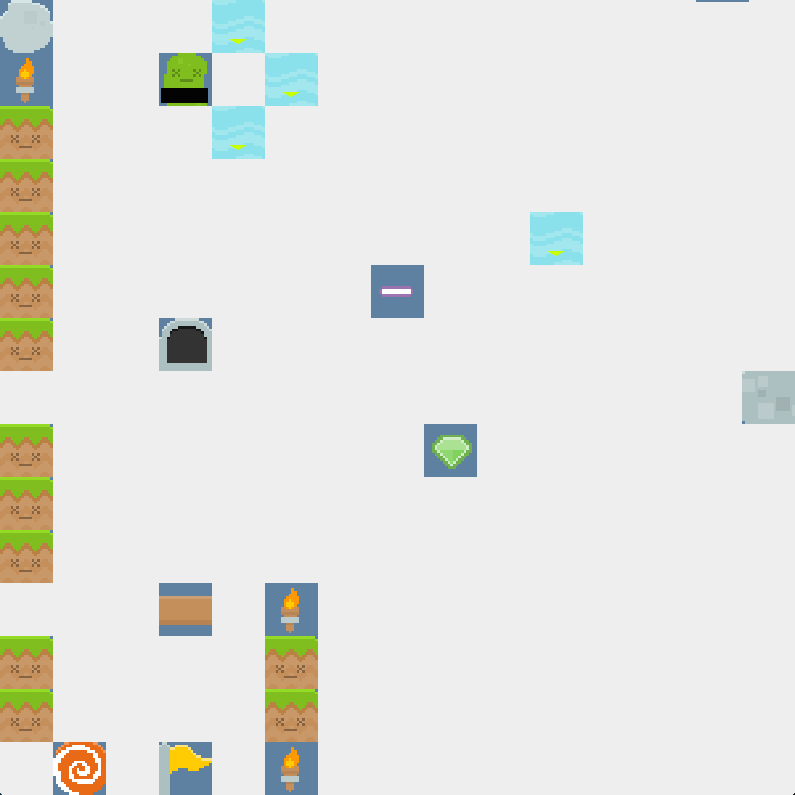
\includegraphics[width=0.45\textwidth]{gengame.png}
	\caption{Visual representation of one of the 400 randomly generated VGDL games}
\end{figure}

Before generating descriptions, we used similar constraints to those mentioned in section~\ref{method:mutation}, partly to avoid generating descriptions with invalid elements, and partly to increase the proportion of interesting outcomes. 
The number of sprites, interaction- and termination-rules were randomly chosen, limited to 25, 25, and 2, respectively. Furthermore, a simple level description (only containing one of each sprite) was generated for each of the generated game descriptions for test purposes. 


%---------------------------------------------------------------

\section{Results}
\label{sec:result}
%Gabriella
The seven controllers mentioned in section \ref{method:controllers} were used to play through a set of example-, mutated and randomly generated games. Because of CPU budget limitations, each game was played for a maximum of 200 clock ticks, and each controller was restricted to use 50 ms on each tick. In the following sections, we show results of these tests, analyze the average of all play-throughs for each controller, and compare the results with each other.

To more accurately compare the score for the different controllers across the range of different games, we normalise each score using a max-min normalisation. 
Normalised averages and win rate averages are shown in Figures \ref{graph:maxminmean} and \ref{graph:winrate}, respectively. In Figure \ref{graph:maxminmean}, it is possible to see that the difference between the highest and lowest scores is greater in the example and mutated games than in the generated games. On the other hand, the average win rate of generated games surpasses both examples and mutated games, as shown in Figure \ref{graph:winrate}.

In addition to the score and win-rate, the average entropy of actions chosen for the player avatar is shown in the tables below.
%tables, possibly graphs, dry explanations of what we observer here (e.g. dontdie seems to do best in example games)

%4.1
\subsection{Example games}

\begin{figure}[!ht]
\centering
\begin{stripedtabular}{llS[table-format = 3.2, round-mode=places, round-precision=2]S[table-format = 4.2, round-mode=places, round-precision=2]S[table-format = 1.4, round-mode=places, round-precision=4]S[table-format = 1.4, round-mode=places, round-precision=4]S[table-format = 1.4, round-mode=places, round-precision=4]l}  \toprule
\rowcolor{white}&\textbf{\emph{controller}} & \emph{mean} & \emph{std.dev.} & \emph{normalised-mean}  & \emph{winrate} & \emph{act-entropy} &\\\midrule
  \DTLforeach{examplesdata}{
  \agent=Agent:,
  \mean=Mean:,
  \std=Std. deviation:,
  \mmave=MaxMinN-Mean:,
  \wrate=Winrate:,
  \entropy=Actions entropy:}
  {\DTLiffirstrow{}{\tabularnewline}%
  & \agent & \mean  & \std  & \mmave  & \wrate & \entropy &} 
  \\ \bottomrule
\end{stripedtabular}
\caption{Results from the 20 example games}
\label{table:examples}
\end{figure}

Averages and win-rates across the 18 example games are shown in Figure~\ref{table:examples}.
The distributions of normalized score values show that more intelligent controllers tend to have more success. 
It is worth noticing that the \emph{score mean} and \emph{normalised score mean} have slightly different orderings.
Notice also that distributions are slightly different when analysing the results of individual games. For instance, in \emph{Aliens}, Random has a higher average than Onestep.
 

%table of how all controllers do on (all) these games; z-score normalised score, win rate, stddev, anything else?

%example of how the controllers did on two or three of these games - including numbers in table and textual description

%4.2
\subsection{Mutated example games}

When generating VGDL game description two different problematic type of games appear: Games where the controllers never increase their score (and never win), and games where too many objects are created and each frame end up taking too long ($>50$ms). 
We remove the play through data for both these types of games in the following analysis.

Total averages of playing through the remaning 291 mutated games (of 360)  (\ref{method:mutation}) are shown in Figure \ref{table:mutation}. 
It is visible that the scores all have higher means and standard deviations, indicating outliers in the data. 
The ordering of the \emph{normalised score mean} however show a similar pattern as for the example games, with Explorer again excelling.
%It is possible to notice that, in general, Explorer seems to excel against the others. 
%Onestep-S is second, followed closely by GA and MCTS. 
%With worse averages, Random, DoNothing and, surprisingly, Onestep-H are, respectively, the worse. 
%It is also visible that average scores are considerably higher that those obtained in the example games.

\begin{figure}[!ht]
\centering
\begin{stripedtabular}{llS[table-format = 3.2, round-mode=places, round-precision=2]S[table-format = 4.2, round-mode=places, round-precision=2]S[table-format = 1.4, round-mode=places, round-precision=4]S[table-format = 1.4, round-mode=places, round-precision=4]S[table-format = 1.4, round-mode=places, round-precision=4]l}  \toprule
\rowcolor{white}&\textbf{\emph{controller}} & \emph{mean} & \emph{std.dev.} & \emph{normalised-mean}  & \emph{win-rate} & \emph{act-entropy} &\\\midrule
  \DTLforeach{mutateddata}{
  \agent=Agent:,
  \mean=Mean:,
  \std=Std. deviation:,
  \mmave=MaxMinN-Mean:,
  \wrate=Winrate:,
  \entropy=Actions entropy:}
  {\DTLiffirstrow{}{\tabularnewline}%
  & \agent & \mean  & \std  & \mmave  & \wrate & \entropy &} 
  \\ \bottomrule
\end{stripedtabular}
\caption{Results from mutated games} \label{table:mutation}
\end{figure}


%table of how all controllers do on (all) mutated games; z-score normalised score, win rate, stddev, anything else?

%example of what mutations could happen

%any observations?
%4.3
\subsection{Randomly generated games}
As for the mutated example games, problematic games were removed from the set leaving 86 games (shown in Figure \ref{table:generated}).

First of all, \emph{score means} are much higher than in the previous games, with the minimum average being 383.96, 8.5 times bigger than the higher mean in the mutated games (i.e. 45.22, by the Explorer).
The ordering of controllers according to the \emph{score mean} has also changed, with Onestep-H on top followed by GA. 
The \emph{normalised score means} and \emph{win-rates} have more similar values than the previous games 
%It is, from higher to lower, Onestep-H $>$ GA $>$ MCTS $>$ DoNothing $>$ Explorer $>$ Onestep-S $>$ Random.


\begin{figure}[!ht]
\centering
\begin{stripedtabular}{llS[table-format = 3.2, round-mode=places, round-precision=2]S[table-format = 4.2, round-mode=places, round-precision=2]S[table-format = 1.4, round-mode=places, round-precision=4]S[table-format = 1.4, round-mode=places, round-precision=4]S[table-format = 1.4, round-mode=places, round-precision=4]l}  \toprule
\rowcolor{white}&\textbf{\emph{controller}} & \emph{mean} & \emph{std.dev.} & \emph{normalised-mean}  & \emph{win-rate} & \emph{act-entropy} &\\\midrule
  \DTLforeach{generateddata}{
  \agent=Agent:,
  \mean=Mean:,
  \std=Std. deviation:,
  \mmave=MaxMinN-Mean:,
  \wrate=Winrate:,
  \entropy=Actions entropy:}
  {\DTLiffirstrow{}{\tabularnewline}%
  & \agent & \mean  & \std  & \mmave  & \wrate & \entropy &} 
  \\ \bottomrule
\end{stripedtabular}
\caption{Results from randomly generated games}\label{table:generated}
\end{figure}

%table of how all controllers do on (all) randomly generated games; z-score normalised score, win rate, stddev, anything else?

%characterise the results

%example of how a generated game or two could look like



\begin{figure}[!ht]
\centering
\begin{tikzpicture}[font=\small, scale=1]
  \begin{axis}[
	ybar, bar width=0.38cm,
	xtick=data, xtick pos=left,
	ylabel=Average normalised score, ymajorgrids, ymin=0, ymax=1,
	symbolic x coords={Explorer,MCTS,GA,Onestep-S,Onestep-H, Random, DoNothing},
	width=\textwidth, height=6cm,
	legend style={
	  overlay, area legend, anchor=north,legend columns=1, at={(0.88,1.00)} %, at={(0.5,-0.15)}
	},
	legend image code/.code={%
          \draw[#1, draw=none] (0cm,-0.1cm) rectangle (0.6cm,0.1cm);
        }
]
    \addplot[fill=blue!40, error bars/.cd, y dir=both, y explicit] table [x=Agent:, y=MaxMinN-Mean:, y error=MaxMinN-SE:, col sep=comma] {examplesdata.csv};
    \addplot[fill=red!10, error bars/.cd, y dir=both, y explicit] table [x=Agent:, y=MaxMinN-Mean:, y error=MaxMinN-SE:, col sep=comma] {mutateddata.csv};
    \addplot[fill=red!50, error bars/.cd, y dir=both, y explicit] table [x=Agent:, y=MaxMinN-Mean:, y error=MaxMinN-SE:, col sep=comma] {generateddata.csv};
\legend{examples,mutated,generated}
\end{axis}
\end{tikzpicture}
\caption{Average normalised score}
\label{graph:maxminmean}
\end{figure}

\begin{figure}[!ht]
\centering
\begin{tikzpicture}[font=\small, scale=1]
  \begin{axis}[
	ybar, bar width=0.38cm,
	xtick=data, xtick pos=left,
	ylabel=Average wins, ymajorgrids, ymin=0, ymax=0.26,
	y tick label style={/pgf/number format/precision=2, /pgf/number format/fixed,},
	symbolic x coords={Explorer,MCTS,GA,Onestep-S,Onestep-H, Random, DoNothing},
	width=\textwidth, height=6cm,
	legend style={
	  overlay, area legend, anchor=north,legend columns=1, at={(0.88,1.00)} %, at={(0.5,-0.15)}
	},
	legend image code/.code={%
          \draw[#1, draw=none] (0cm,-0.1cm) rectangle (0.6cm,0.1cm);
        }
]
    \addplot[fill=blue!40, error bars/.cd, y dir=both, y explicit] table [x=Agent:, y=Winrate:, y error=Winrate-SE:, col sep=comma] {examplesdata.csv};
    \addplot[fill=red!10, error bars/.cd, y dir=both, y explicit] table [x=Agent:, y=Winrate:, y error=Winrate-SE:, col sep=comma] {mutateddata.csv};
    \addplot[fill=red!50, error bars/.cd, y dir=both, y explicit] table [x=Agent:, y=Winrate:, y error=Winrate-SE:, col sep=comma] {generateddata.csv};
\legend{examples,mutated,generated}
\end{axis}
\end{tikzpicture}
\caption{Average wins}
\label{graph:winrate}
\end{figure}

%---------------------------------------------------------------

\section{Discussion}
%Julian and Mark

The results in Section~\ref{sec:result} display some interesting patterns. Win rates suggest a relationship between intelligent controllers' success and better game design, corroborating our original hypothesis. In randomly generated games, which arguably tend to be less interesting than the others, smarter controllers (e.g. Explorer and MCTS) do only slightly better than the worse ones (i.e. Random and DoNothing). This is due to a general a lack of consistency between rules generated in this manner. Mutated games, however, derive from a designed game. Therefore, they maintain some characteristics of the original idea, which can improve the VGDL description's gameplay and playability.

A t-test was performed to determine the difference between the set of example- and generated games. Using the relative score-difference between the controllers Explorer and Random, the two distributions are drawn from different sets with a $p$-value of $\le 0.0001$.

The contrast in scores between smarter and dumber controllers is smaller in generated games than the example ones. However, in the random generation process, score values attributed to actions are also chosen at random. This possibly impacted the outcome of this results, decreasing the discrepancy between scores.
Furthermore, it is interesting that Random and DoNothing do well in some games, as seen in Figure~\ref{graph:winrate}. While it is possible that random actions can result in good outcomes, this chance is very low, especially when compared to the chance of making informated decisions. In spite of that, Random does fairly well in randomly generated games. DoNothing does even better. While in example games it never wins, it does so, albeit rarely, in mutated ones. But in randomly generated games, it performs even better than Onestep-S and Random, which we believe indicates quite poor design of the randomly generated games.


\section{Conclusion}
%Julian
Our intent has been to investigate evaluating video games via the performance of game-playing algorithms. We hypothesized that the performance difference between good and bad game-playing algorithms is higher on well-designed games, and therefore can be used as at least a partial proxy for game quality. To test this theory, we had seven controllers with varying levels of skill play 18 human-designed, 291 mutated, and 86 randomly generated VGDL games. The results seem to corroborate our initial conjecture, showing a clear distinction between results of more and less intelligent controllers across the games, with the difference decreasing as the games' qualities decrease.

We also suggest new controllers for GVG-AI: Explorer, OneStep-Score and DoNothing. The first one in particular shows strong overall performance compared to existing baselines such as ``vanilla'' MCTS.


\begin{figure}[!ht]
\centering
\begin{stripedtabular}{llS[table-format = 3.2, round-mode=places, round-precision=2]S[table-format = 4.2, round-mode=places, round-precision=2]S[table-format = 1.4, round-mode=places, round-precision=4]S[table-format = 1.4, round-mode=places, round-precision=4]S[table-format = 1.4, round-mode=places, round-precision=4]l}  \toprule
\rowcolor{white}&\textbf{\emph{controller}} & \emph{mean} & \emph{std.dev.} & \emph{normalised-mean}  & \emph{winrate} & \emph{act-entropy} &\\\midrule
  \DTLforeach{examplesdata}{
  \agent=Agent:,
  \mean=Mean:,
  \std=Std. deviation:,
  \mmave=MaxMinN-Mean:,
  \wrate=Winrate:,
  \entropy=Actions entropy:}
  {\DTLiffirstrow{}{\tabularnewline}%
  & \agent & \mean  & \std  & \mmave  & \wrate & \entropy &} 
  \\ \bottomrule
\end{stripedtabular}
\caption{Results from the 20 example games}
\label{table:examples}
\end{figure}



% TODO
%  add acknowledgments section
%  acknowledge gabriella's grant
%  maybe acknowledge the GVGAI people

\bibliography{bigliography}
\bibliographystyle{splncs03}
\end{document}